\section{Results}

\subsection{Aliasing Distortion}

\begin{figure}[H]
    \centering
    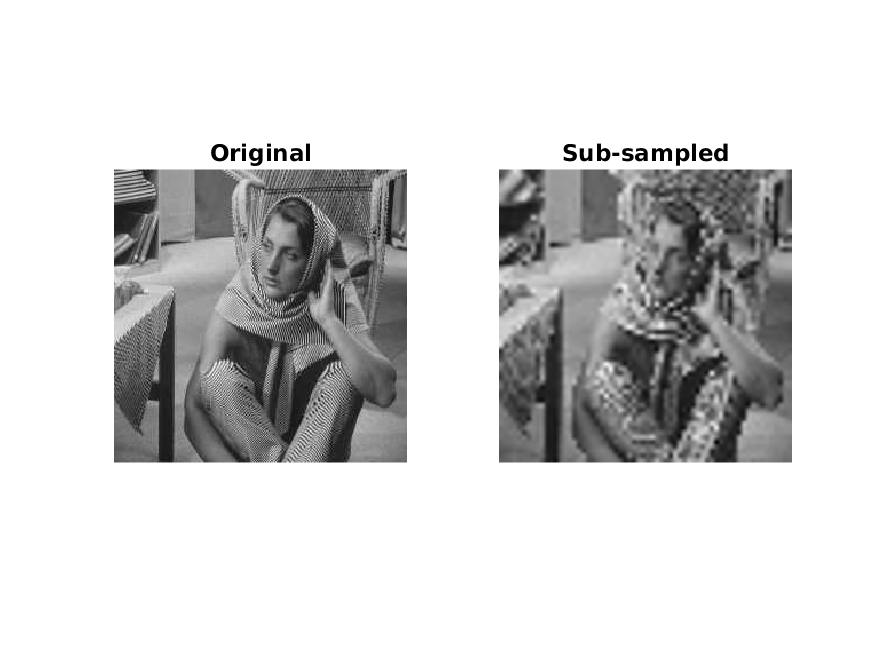
\includegraphics[scale=0.75]{sub_sampled.png}
    \caption{Sub-sampling barabara}
\end{figure}

\begin{figure}[H]
    \centering
    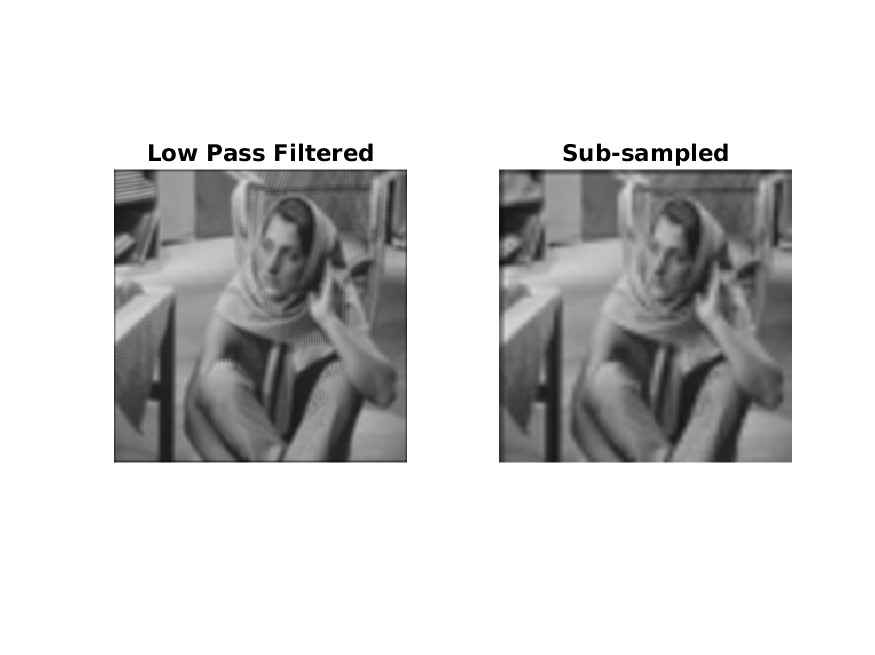
\includegraphics[scale=0.75]{low_pass_sub_sampled.png}
    \caption{Sub-sampling loe-passed barbara}
\end{figure}

Sub-sampling creates a noticeable amount of distortion. This is due to the fact
that the larger the spacing of samples means that the spectral images become
closer. As these overlap, there is aliasing, and therefore distortion. In our
first image we can see that as we view the sub-sampled image of barabara.

In our second image we put barbara through a low pass filter. This effectively
removes high frequencies and shrinks the spectral image. We get the same
spectral spacing as before, however the spectral images do not overlap and we do
not get any aliasing. As seen above, there is little difference before and after
sub-sampling.

\subsection{Formula Based Image Sampling}

\begin{figure}[H]
    \centering
    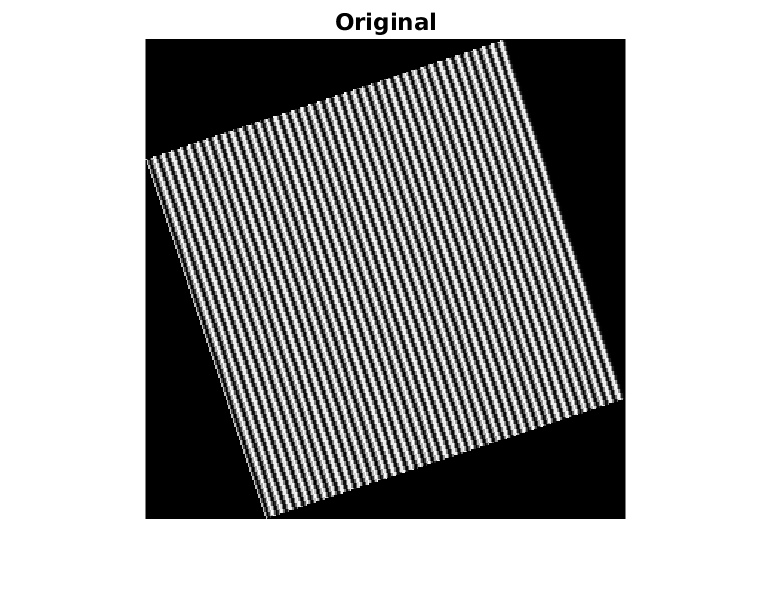
\includegraphics[scale=0.75]{original_sine.png}
    \caption{Image with single frequency in x and y axis}
\end{figure}

\begin{figure}[H]
    \centering
    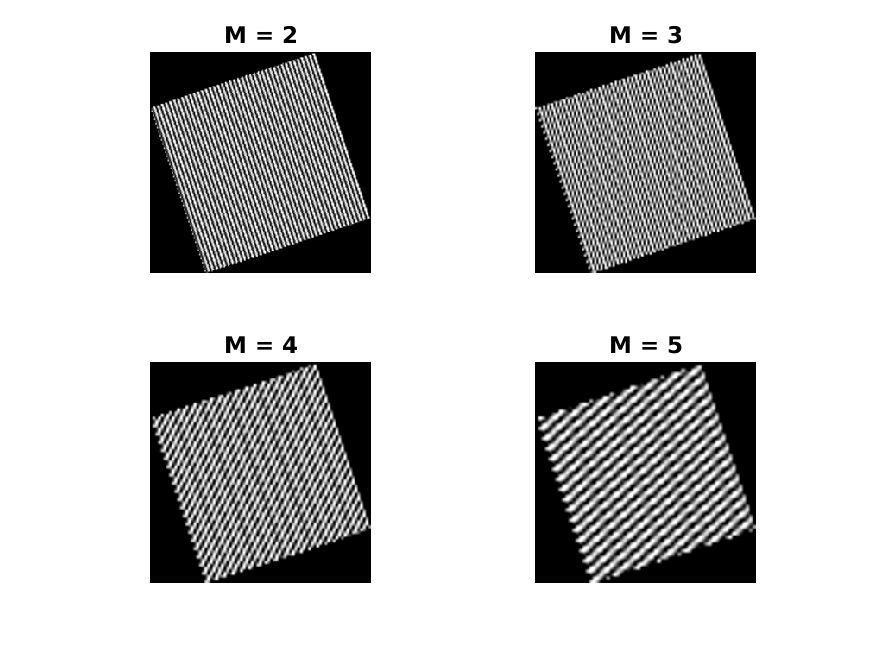
\includegraphics[scale=0.75]{sub_sample_sine.png}
    \caption{Sub-sampled sine image}
\end{figure}

Here we have created an image with a single frequency in the x axis, and another
single frequency in the y axis. We sub-sample this image under different values
of M. This then resulted in different spacing of the spectral images, and
differences in aliasing. We can see this take effect as the lines seem to
rotate as we increase the sample spacing.
